\documentclass{beamer}
\usetheme{Madrid}



\begin{document}
%导言区
\title{Compile to JVM}
\author{Jiawei Chen, Zhetuo Qi}
\institute{Zhejiang University}
%正文
\begin{frame}
    \maketitle
\end{frame}

\begin{frame}
    \frametitle{Language Specification}
    \begin{figure}[h]
        \centering
        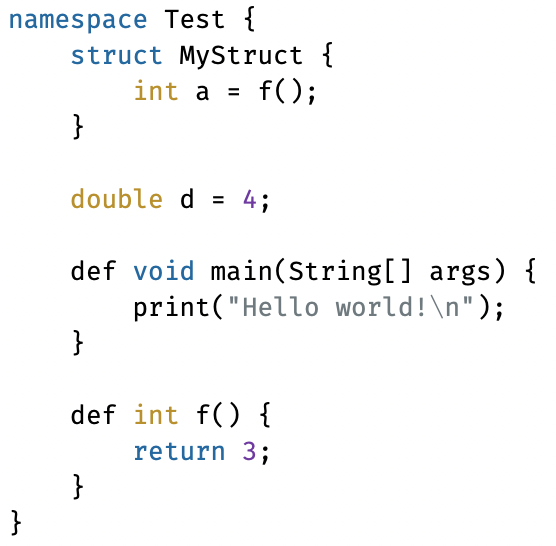
\includegraphics[scale=0.7]{assets/general.png}    
    \end{figure}
\end{frame}

\begin{frame}
    \frametitle{Compiler Architecture}
    \begin{figure}[h]
        \centering
        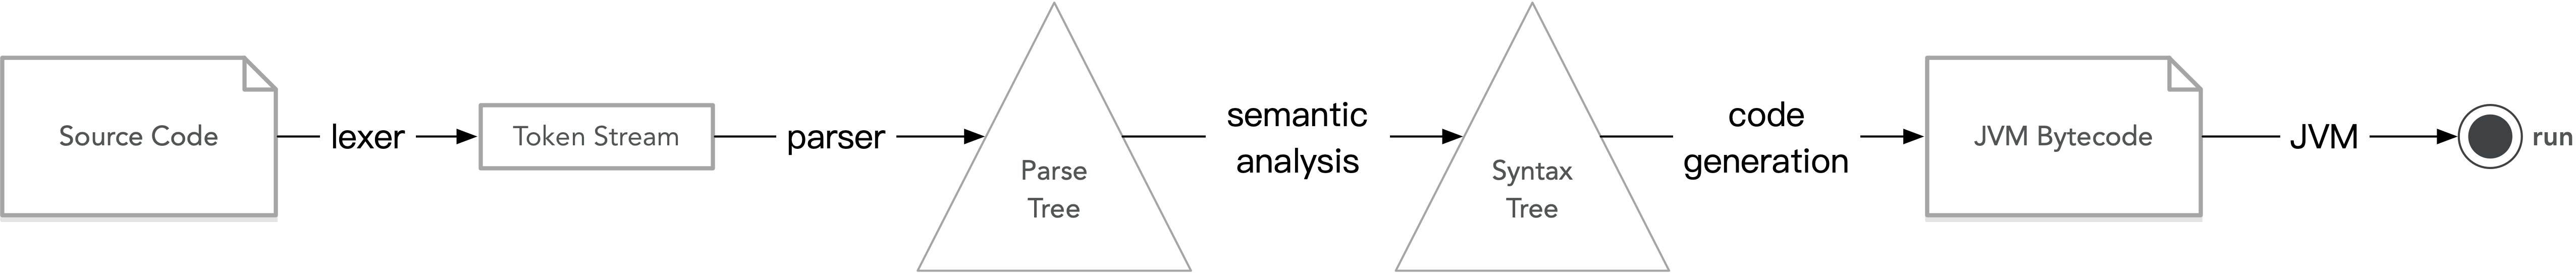
\includegraphics[scale=0.28]{assets/architecture.png}    
    \end{figure}
\end{frame}

\begin{frame}
    \frametitle{Third Party Library}
    \begin{itemize}
        \item commons-cli: parse the command line
        \item ANTLR 4: lexical/syntactic analysis
        \item ASM: help to generate Java bytecode
    \end{itemize}
\end{frame}

\begin{frame}
    \frametitle{Lexical Analysis}
    By ANTLR, we can write the following rules:
    % TODO: code of antlr
\end{frame}

\begin{frame}
    \frametitle{Syntactic Analysis}
    By ANTLR, we can write the following parsing rules, all the rules are placed in a .g4 file.
    % TODO: code of antlr
    Note: ANTLR doesn't support left-recursive, we have to solve it manually.
\end{frame}


\begin{frame}
    \frametitle{Syntactic Analysis}
    \begin{figure}[h]
        \centering
        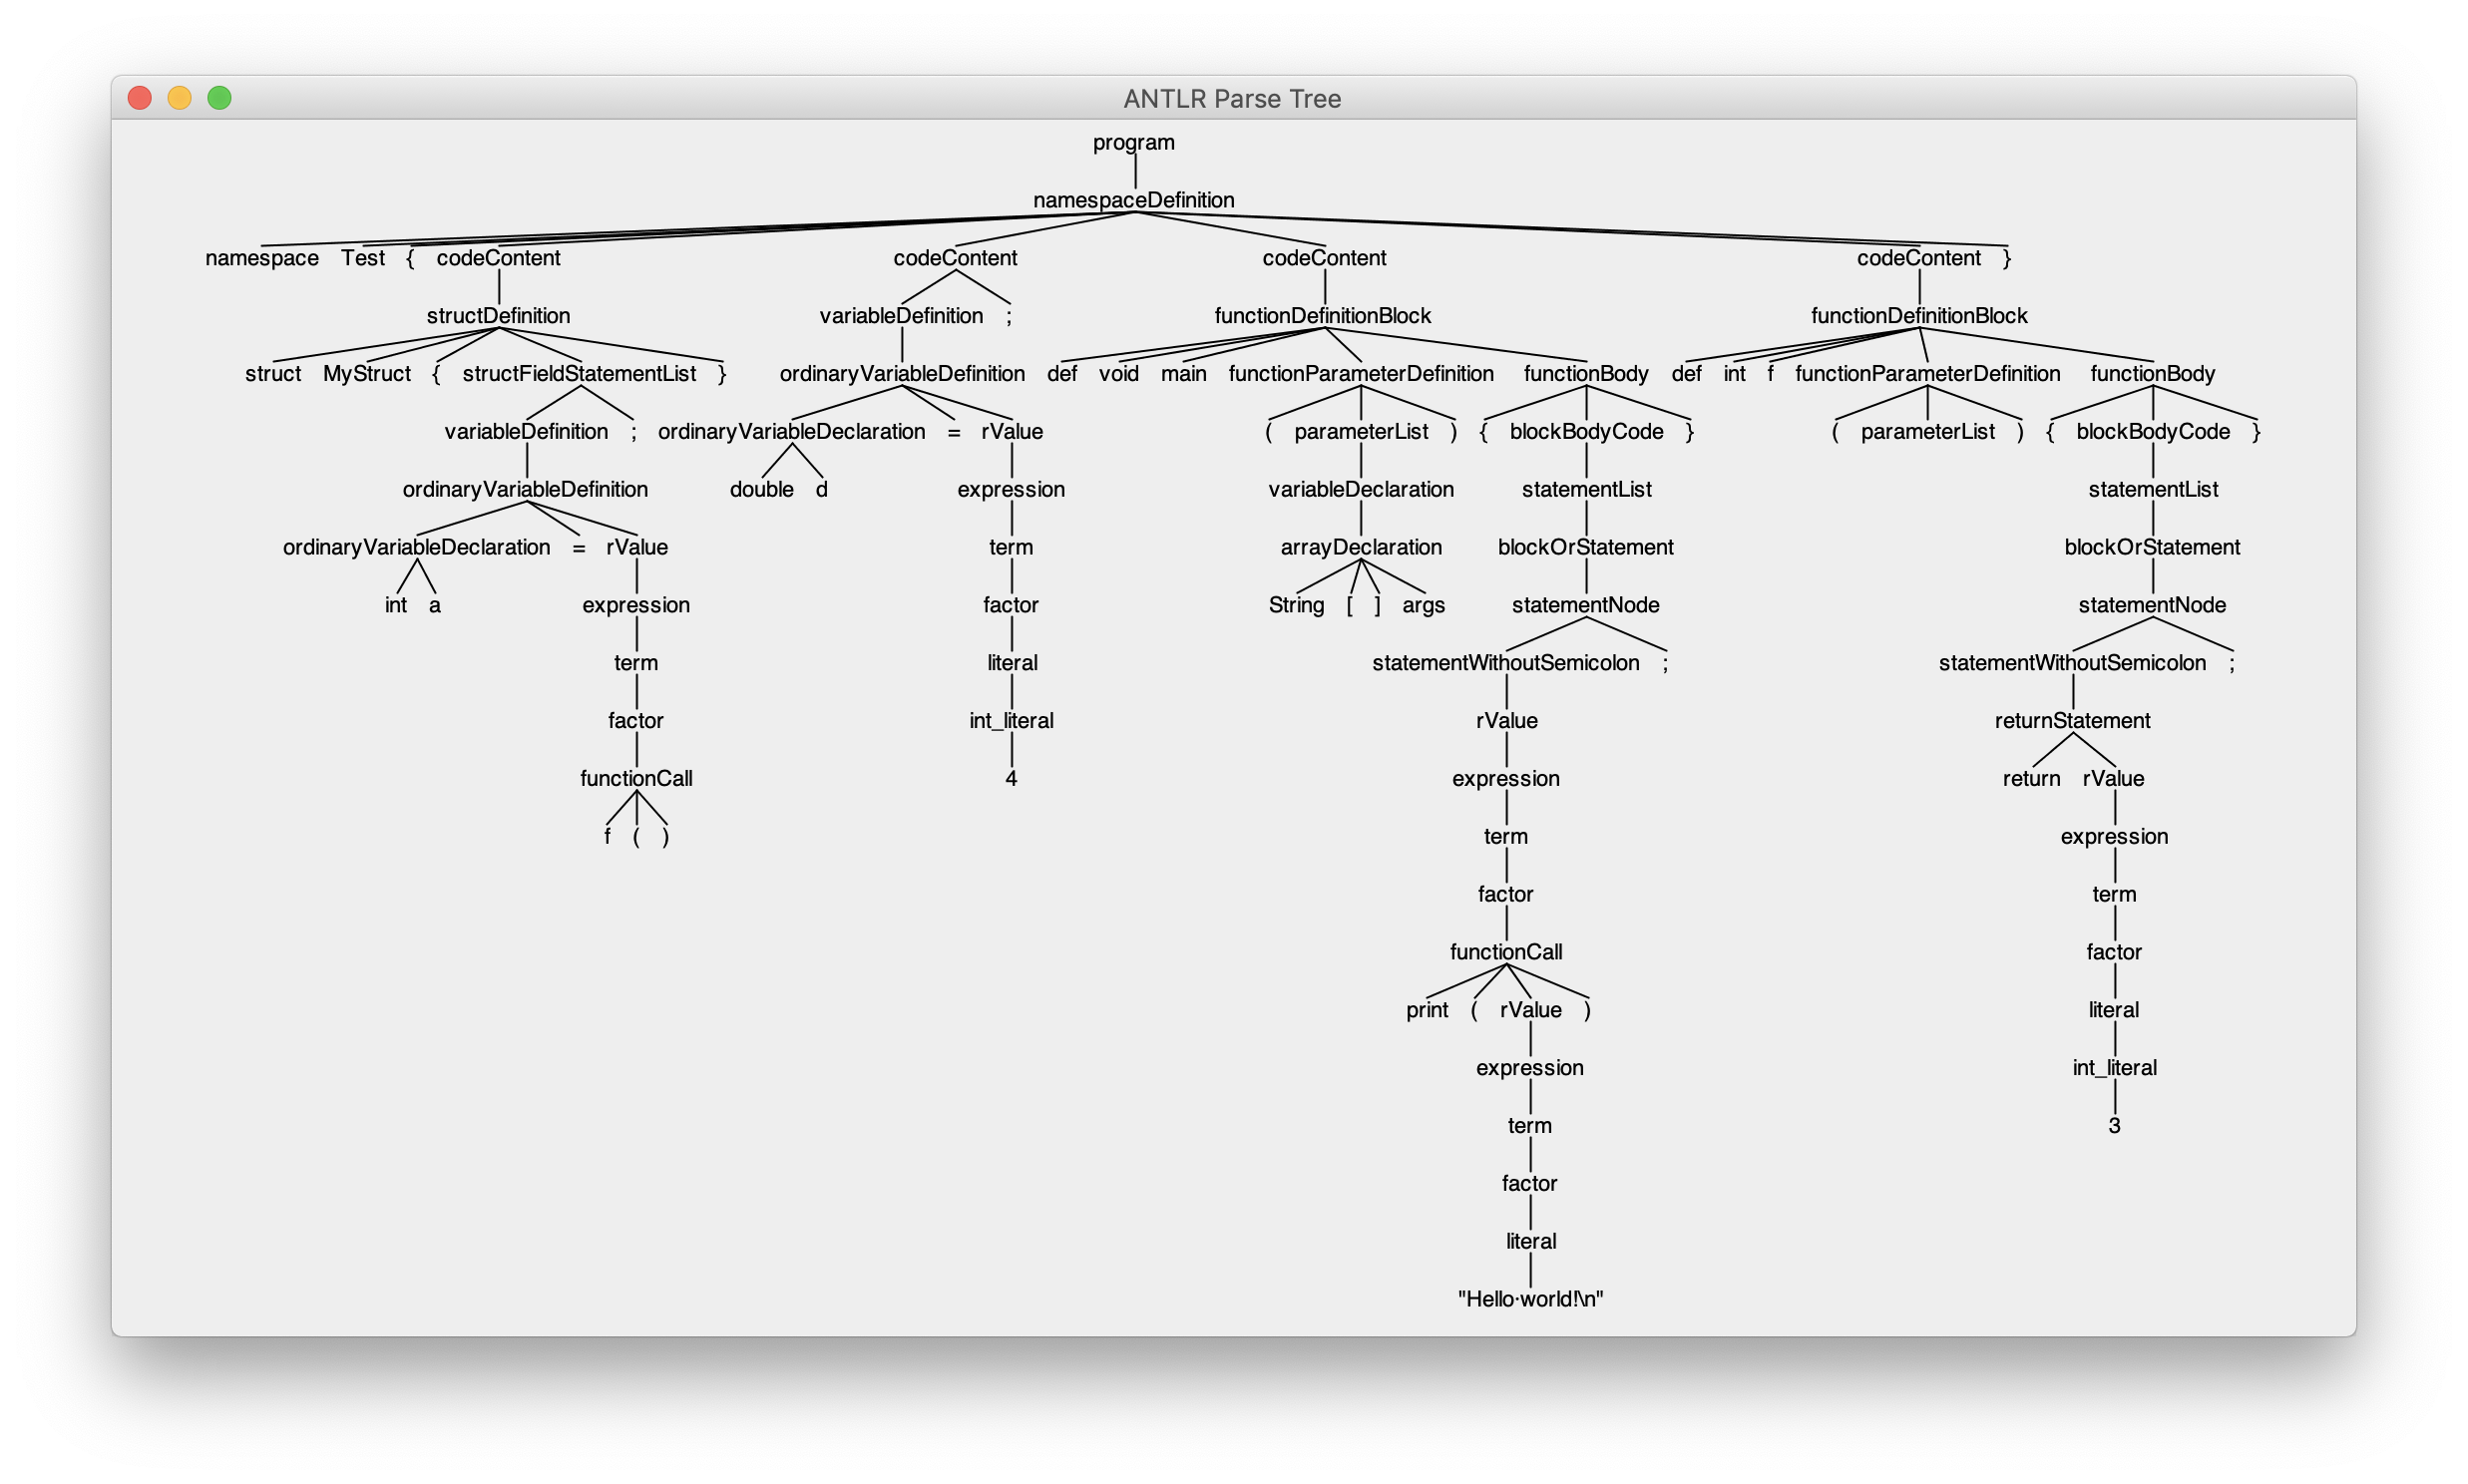
\includegraphics[scale=0.28]{assets/ParseTree.png}
    \end{figure}
\end{frame}

\begin{frame}
    \frametitle{Semantic Analysis}
    \begin{figure}[h]
        \centering
        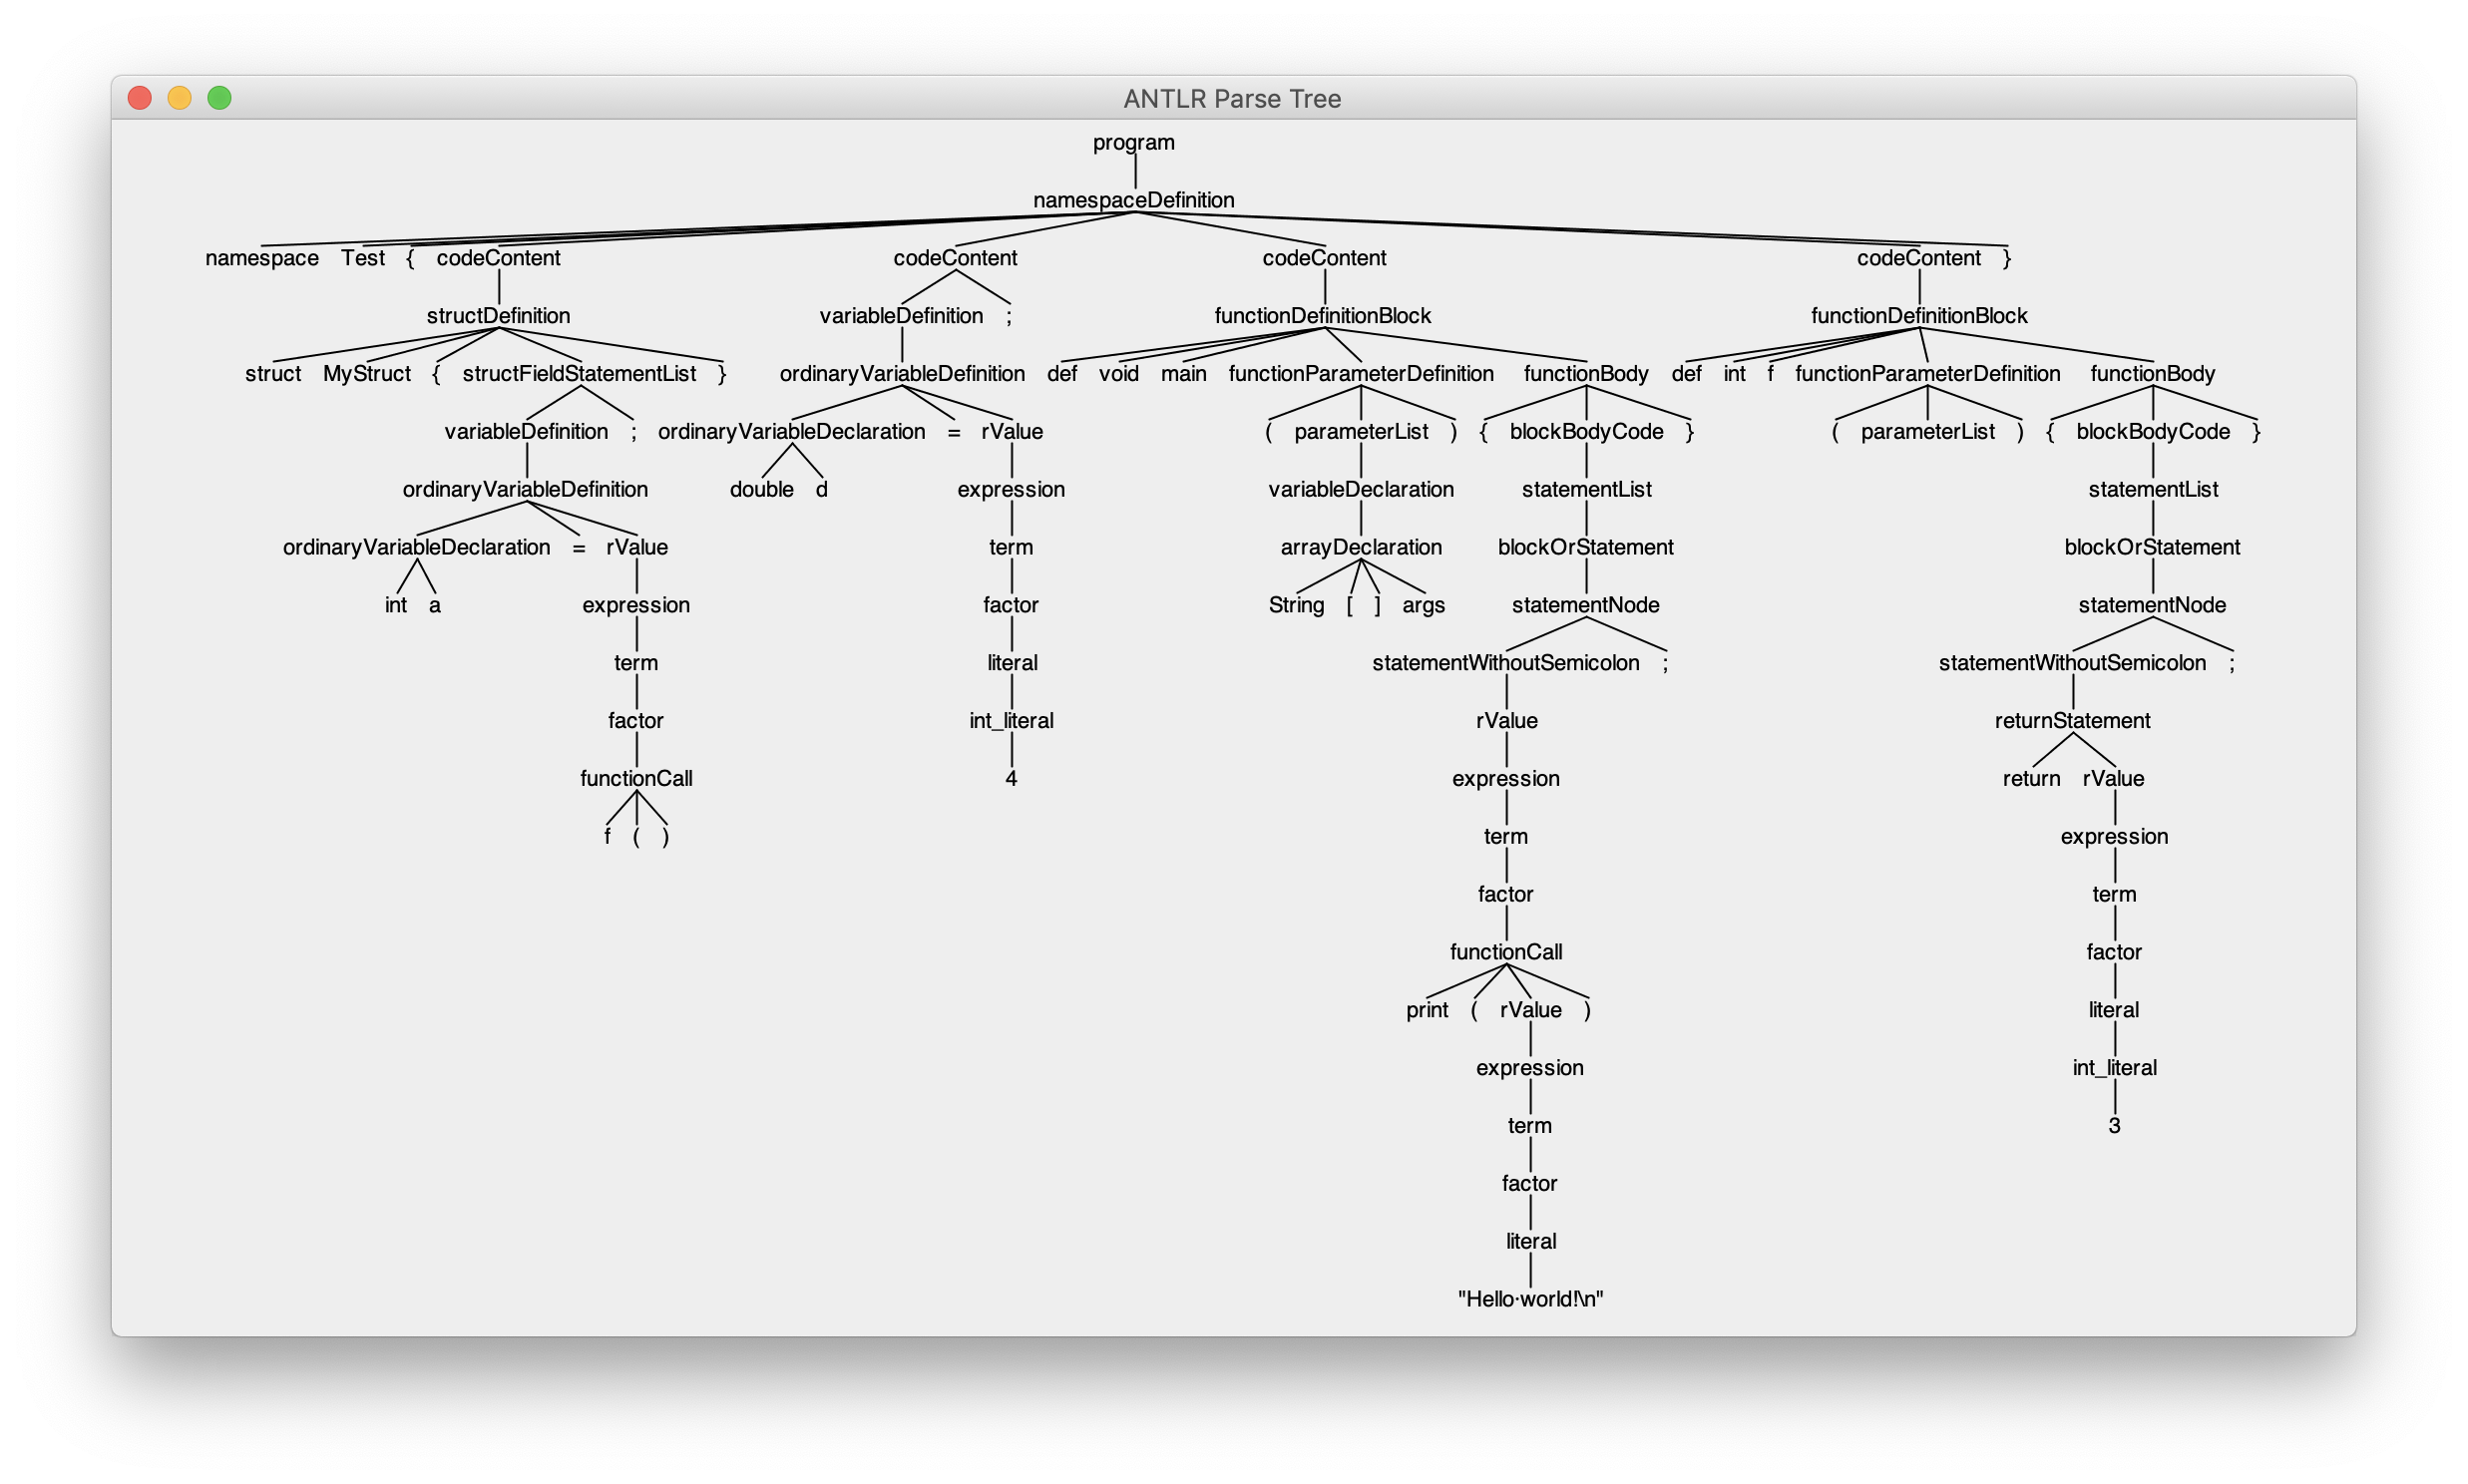
\includegraphics[scale=0.28]{assets/ParseTree.png}
    \end{figure}
\end{frame}

\begin{frame}
    \frametitle{Type I and Type II Errors}
    \begin{block}{False Negative Errors}
        A false negative is an error in which a test/study result is negative but in reality it is positive.
    \end{block}
\end{frame}



\begin{frame}
    \begin{block}{True Positive Rate, TPR}
        \begin{equation}
            TPR=\frac{TP}{TP+FN}
        \end{equation}
    \end{block}
    
    \begin{block}{False Positive Rate, FPR}
        \begin{equation}
            FPR=\frac{FP}{FP+TN}
        \end{equation}
    \end{block}
    
%    \begin{figure}[h]
%        \centering
%        \includegraphics[scale=0.2]{error.jpg}    
%    \end{figure}
\end{frame}

\begin{frame}
    \frametitle{ROC Space}
    \begin{block}{True Positive Rate, TPR}
        \begin{equation}
            TPR=\frac{TP}{TP+FN}
        \end{equation}
    \end{block}
    
    \begin{block}{False Positive Rate, FPR}
        \begin{equation}
            FPR=\frac{FP}{FP+TN}
        \end{equation}
    \end{block}
    
    \begin{block}{ROC Space}
        An ROC space is defined by \textbf{FPR} and \textbf{TPR} as $x$ and $y$ axes, respectively, which depicts relative trade-offs between true positive (benefits) and false positive (costs)
    \end{block}
    
\end{frame}

\begin{frame}
    \vspace{-1cm}
    \begin{figure}[h]
        \centering
        \includegraphics[scale=0.45]{ROC_space-2.png}    
    \end{figure}
    \vspace{-1cm}
    \begin{itemize}
        \item[$\blacksquare$] Each prediction result represents one point in the ROC space.
    \end{itemize}
\end{frame}

\begin{frame}
    \vspace{-1cm}
    \begin{figure}[h]
        \centering
        \includegraphics[scale=0.45]{ROC_space-2.png}    
    \end{figure}
    \vspace{-1cm}
    \begin{itemize}
        \item[$\blacksquare$] What if a result point locates in the diagonal line?
    \end{itemize}
\end{frame}

\begin{frame}
    \begin{block}{Accuracy}
        \begin{equation}
            Accuracy=\frac{TP + TN}{TP + FP + FN + TN}
        \end{equation}
    \end{block}
    \begin{figure}[h]
        \centering
        \includegraphics[scale=0.25]{error.jpg}    
    \end{figure}
\end{frame}

\begin{frame}
    \begin{itemize}
        \item[$\blacksquare$] Suppose the number of positive results equals to the number of negative results in reality.
    \end{itemize}
    \begin{equation}
        TP + FN = FP + TN
    \end{equation}
    \begin{itemize}
        \item[$\blacksquare$] Then a result point located in the diagonal line means:
    \end{itemize}
    \begin{equation}
        \begin{aligned}
            \frac{TP}{TP+FN} &= \frac{FP}{FP+TN} \\
            \Rightarrow Accuracy &= \frac{TP + TN}{TP + FP + FN + TN} = 50\%
	      \end{aligned}
    \end{equation}
    \begin{itemize}
        \item[$\blacksquare$] So the diagonal line are called line of no-discrimination (line of random guess)
    \end{itemize}
\end{frame}


\begin{frame}
    \vspace{-1cm}
    \begin{figure}[h]
        \centering
        \includegraphics[scale=0.45]{ROC_space-2.png}    
    \end{figure}
    \vspace{-1cm}
    \begin{itemize}
        \item[$\blacksquare$] The result located in the diagonal line has 50\% accuracy
    \end{itemize}
\end{frame}

\begin{frame}
    \vspace{-1cm}
    \begin{figure}[h]
        \centering
        \includegraphics[scale=0.45]{ROC_space-2.png}    
    \end{figure}
    \vspace{-1cm}
    \begin{itemize}
        \item[$\blacksquare$] The closer a result is to the upper left corner, the better it predicts.
        \item[$\blacksquare$] The closer a result is to the lower right corner, the worse it predicts.
    \end{itemize}
\end{frame}

\begin{frame}
    \frametitle{ROC Curves}
    \begin{block}{ROC Curve}
        Fix binary classifier model and change the threshold, the result points will generate the ROC curve.
    \end{block}
    \begin{exampleblock}{Example}
        \begin{figure}[h]
            \centering
            \includegraphics[scale=0.3]{ROC-example.jpg}    
        \end{figure}    
    \end{exampleblock}
\end{frame}

\begin{frame}
    \frametitle{AUC}
    \begin{block}{AUC}
        Area under the curve of ROC curve.
    \end{block}
    \begin{exampleblock}{Example}
        \begin{figure}[h]
            \centering
            \includegraphics[scale=0.6]{AUC.png} 
        \end{figure}    
    \end{exampleblock}
    \begin{itemize}
        \item[$\blacksquare$] $AUC \leqslant 1$
    \end{itemize}
\end{frame}

\begin{frame}
    \begin{exampleblock}{Example}
        \begin{figure}[h]
            \centering
            \includegraphics[scale=0.6]{AUC-examples.png}
        \end{figure}    
    \end{exampleblock}
    
    \begin{itemize}
        \item[$\blacksquare$] $AUC = 1$, perfect classifier
        \item[$\blacksquare$] $0.5 < AUC < 1$, better than random guess
        \item[$\blacksquare$] $AUC = 0.5$, same as random guess
        \item[$\blacksquare$] $AUC < 0.5$, worse than random guess
    \end{itemize}
\end{frame}

\begin{frame}
    \frametitle{Balance of FPR and FNR}
    
    \begin{itemize}
        \item[$\blacksquare$] With the decrease of FPR, FNR increases.
    \end{itemize}
    
    \begin{exampleblock}{Example}
        \begin{figure}[h]
            \centering
            \includegraphics[scale=0.35]{ROC-example.jpg}    
        \end{figure}    
    \end{exampleblock}
\end{frame}

\begin{frame}
    \frametitle{Balancing according to concrete situations}
    
    \begin{itemize}
        \item[$\blacksquare$] \textbf{Prediction of earthquakes:} we prefer to predict every earthquake successfully, which means that we can tolerate the increase of FPR compared to FNR.
    \end{itemize}
    \begin{figure}[h]
        \centering
        \includegraphics[scale=0.2]{Earthquake.png}   
    \end{figure} 
\end{frame}

\begin{frame}
    \frametitle{Balancing according to concrete situations}
    
    \begin{itemize}
        \item[$\blacksquare$] \textbf{Conviction:} By the presumption of innocence, we prefer to be cautious when involving criminal justice, so we have to tolerate larger FNR compared to FPR.
    \end{itemize}
    \begin{figure}[h]
        \centering
        \includegraphics[scale=0.35]{prisoner.jpeg}
    \end{figure} 
\end{frame}

%\begin{frame}
%    \begin{itemize}
%        \item[$\blacksquare$] Fawcett, Tom (2006). "An Introduction to ROC Analysis" (PDF). Pattern Recognition Letters. 27 (8): 861–874. doi:10.1016/j.patrec.2005.10.010
%    \end{itemize}
%\end{frame}

\end{document}
